\section{Object definition and selection}

  All lepton, jet and \met objects in the event are reconstructed using the Particle Flow (PF) algorithm~\citep{CMS-PAS-PFT-09-001}.
  Jets are corrected for by {\texttt Spring16\_25nsV6} corrections and and propagated to \ETmiss (type-1 corrections). 
  \subsection{Lepton selection}
    Leptons are selected according to a set of identification and isolation criteria which are summarized in Table~\ref{leptonSelection} and discussed in the following.
    The leading lepton is required to have a transverse momentum of at least 25 \GeV, while the trailing lepton must exceed 20 \GeV.
    Both leptons must satisfy $-2.4 < \eta < 2.4$. 
    Events with additional leptons satisfying $p_T> 15$ GeV and with relative isolation below 0.4 are vetoed.

    % In case 3rd lepton is vetoed by a loose selection
\begin{table}
  \center
  \small
  \begin{tabular}{c|cc|cc}
                     & \multicolumn{2}{c|}{dilepton selection}            & \multicolumn{2}{c}{3rd lepton veto} \\
                     & electrons                   & muons               & electrons                   & muons \\
     \hline
     \pt             & $> 20\GeV$                  & $> 20\GeV$          & $> 15\GeV$                  & $>15\GeV$ \\
     $|\eta|$        & $< 2.4$                     & $< 2.4$             & $< 2.4$                     & $< 2.4$  \\ 
     isolation       & relIso03 $< 0.12$            & relIso03 $< 0.12$    & relIso03 $< 0.4$            & relIso03 $< 0.4$\\
     $|d_{xy}|$      & $< 0.05$                    & $< 0.05$            & $< 0.05$                    & $< 0.05$    \\
     $|d_{z}|$       & $< 0.1$                     & $< 0.1$             & $< 0.1$                     & $< 0.1$  \\
     SIP3D           & $< 4$                       & $< 4$               & $< 4$                       & $< 4$ \\
     identification  & cut-based tight id          & medium muon id      & cut based veto id           & veto muon id \\
                     & lostHits = 0                &                     &                             &\\ 
  \end{tabular}
  \caption{Lepton selection criteria}
  \label{leptonSelection}
\end{table}


    \subsubsection{Electron identification}
      Electrons need to pass the tight cut-based POG recommended working point in the 25ns scenario~\citep{twiki:eleId} which includes the
      requirement to pass the conversion veto. Additionally, on some identification variables we apply tighter cuts with respect to the official working point. Electron candidates 
      are only considered when they have exactly 0 missing hits. The longitudinal impact parameter $|dz|$ with respect to the primary vertex
      is required to be less than 1\mm in the endcap region ($1.479 < |\eta| < 2.4$). % Note: other impact parameters in the cut-based tight id are dxy < 0.111mm and dz < 0.466mm in the barrel and dxy < 0.351 mm; all which are tighter than our 0.5mm and 1mm
      Additionally, the significance of the 3D impact parameter should satisfy $\text{SIP}_\text{3D} \equiv \left| \frac{\text{IP}}{\sigma_\text{IP}} \right| < 4$ 
      where IP is the distance of closest approach of the lepton track to the event primary vertex and $\sigma_\text{IP}$ is its associated uncertainty. 

    \subsubsection{Muon identification}
      Muons have to pass the medium identification working point \citep{twiki:muonID}. Additionally, the transverse impact parameter $|dxy|$ and the longitudinal impact parameter $|dz|$ with respect to the primary vertex
      are required to be less than 0.5\mm and 1\mm respectively. In the same way as for electrons, the $\text{SIP}_\text{3D}$ is required to be less than 4.

    \subsubsection{Lepton isolation}
      Relative isolation smaller than 0.12 within a cone R of 0.3 around the lepton candidate is required for both electrons and muons.
      We apply the very tight (VT) multi-isolation working point to both electrons and muons. The multi-isolation approach was earlier presented in~\citep{CMS_NOTE_2015-133} and is constructed from three observables:
      \begin{itemize}
        \item the mini-isolation $I_\text{mini}$, defined as
              \begin{equation}
                I_\text{mini} = \frac{\sum_R \pt(h^\pm) + \text{max}\left(0, \sum_R \pt(h^0)+\pt(\gamma) - \rho\mathcal{A}\left(\frac{R}{0.3}\right)^2\right)}{\pt(\ell)},
              \end{equation}
              where $\sum_R\pt(h^\pm)$, $\sum_R\pt(h^0)$ and $\sum_R\pt(\gamma)$ are the sum of the transverse momentum of the charged hadrons, neutral hadrons and photons, respectively, within a cone $R$
              dependent on the lepton \pt:
              \begin{equation}
                  %R = \frac{10}{\text{min}(\text{max}(\pt(\ell), 50), 200)}
                  R = \begin{cases}
		    0.2          & \text{if } \pt < 50\GeV \\
		    10\GeV/\pt   & \text{if } 50 < \pt < 200\GeV \\
		    0.05         & \text{if } \pt > 200\GeV
                  \end{cases}
              \end{equation}
              Using a variable cone size depending on the lepton \pt ensures that the lepton is locally isolated, even in boosted topologies.
              The last term is the so-called effective area correction to mitigate the impact of pileup, where $\rho$ is the pileup energy density, % (fixedGridRhoFastJetAll)
              and the effective areas $\mathcal{A}$ used are listed in Table~\ref{table:effArea}.
              % Spring15dr POG approved areas
\begin{table}
 \begin{center}
   \small
   \begin{tabular}{lc|lc}
     $|\eta|$ range & $\mathcal{A}$(e) & $|\eta|$ range & $\mathcal{A}$($\mu$)  \\
     \hline
     $0.000-1.000$ & 0.1752 & $0.000-0.800$ & 0.0735 \\
     $1.000-1.479$ & 0.1862 & $0.800-1.300$ & 0.0619 \\
     $1.479-2.000$ & 0.1411 & $1.300-2.000$ & 0.0465 \\
     $2.000-2.200$ & 0.1534 & $2.000-2.200$ & 0.0433 \\
     $2.200-2.300$ & 0.1903 & $2.200-2.400$ & 0.0577 \\
     $2.300-2.400$ & 0.2243 & & \\
    %$2.400-2.500$ & 0.2687 & & \\
   \end{tabular}
   \caption{Effective areas used in the mini-isolation calculation for electrons and muons}
   \label{table:effArea}
 \end{center}
\end{table}

        \item the $p_T^\text{ratio}$, which is defined as the ratio of the lepton \pt and the \pt of the closest matched jet, which often contains the lepton itself. 
              If the closest jet is separated more than $\Delta R > 0.4$, then $p_T^\text{ratio} = 1$ is taken. 
              The $p_T^\text{ratio}$ variable is a simple way to identify non-prompt low-\pt leptons originating from low-\pt b-quarks, which fall outside of the mini-isolation cone.
              In order to avoid an over-correction on prompt leptons, the application of the jet energy correction is only applied on the hadronic part of the jet, using the 
              following formula at Lorentz vector level: $j = (j - PU - \ell)*JEC + \ell + PU$, where $\ell$ is the lepton, 
              $PU$ the pileup energy clustered into the jet and $JEC$ the jet energy scale correction to be applied.
        \item the $p_T^\text{rel}$ variable, defined as
              \begin{equation}
                p_T^\text{rel} = \frac{\left(\vec{p}(\text{jet})-\vec{p}(\ell)\right) \cdot \vec{p}(\ell)}{|\vec{p}(\text{jet})-\vec{p}(\ell)|}.
              \end{equation}
              which allows to recover leptons from accidental overlap with jets in boosted topologies. Similarly to $p_T^\text{ratio}$, the jet energy scale corrections are only applied on the hadronic part of
              the considered jet.
      \end{itemize}
      Using those three variables, the multi-isolation VT working point is passed when the following condition is respected:
      \begin{equation}
        I_\text{mini} < 0.09 \wedge ( p_T^\text{ratio} > 0.84 \vee p_T^\text{rel} > 7.2 )
      \end{equation}
      The logic behind this condition is that in addition to being locally isolated by $I_\text{mini}$, the lepton should carry the major part of the energy of the corresponding jet. If the $p_T^\text{ratio}$ does
      not pass the threshold, the lepton is still recovered if the overlap with the jet is accidental which is decided by the $p_T^\text{rel}$ requirement.
      For reference, the multi-isolation working points used in the SUSY group are summarized in Table~\ref{table:multiIsoWP}.
      % Multi-Iso WP 
\begin{table}
 \begin{center}
   \small
   \begin{tabular}{r|ccc}
     WP & $I_\text{mini}$ & $p_T^\text{ratio}$ & $p_T^\text{rel}$  \\
     \hline
     VL & 0.25 & 0.67 & 4.4 \\
     L  & 0.20 & 0.69 & 6.0 \\
     M  & 0.16 & 0.76 & 7.2 \\
     T  & 0.12 & 0.80 & 7.2 \\
     VT & 0.09 & 0.84 & 7.2 \\
   \end{tabular}
   \caption{Multi-isolation working points.}
   \label{table:multiIsoWP}
 \end{center}
\end{table}

    \subsubsection{Lepton selection efficiencies}
      The lepton identification and isolation efficiencies are measured per lepton leg in $Z/\gamma^*\rightarrow \ell\ell$ events using the tag-and-probe technique~\cite{twiki:SF}.
      The resulting data/MC scale factors, derived in bins of lepton \pt and $|\eta|$, have been applied on the MC and are shown in Fig.~\ref{fig:SF_e} for electrons.
      However, the efficiencies in FastSim signal samples are considerably different from those measured in fully simulated samples, due to the different modeling of showers and pileup.
      We therefore apply additional FullSim/FastSim scale factors~\citep{twiki:FSSF} on our signal samples.

      Finally, to address the issue of the loss of hit efficiency due to the Highly Ionizing Particles (HIP) an additional scale factor is applied on each of the lepton legs~\cite{twiki:HIP}.

      \begin{figure}
	\centering
	\subfloat[electron id]{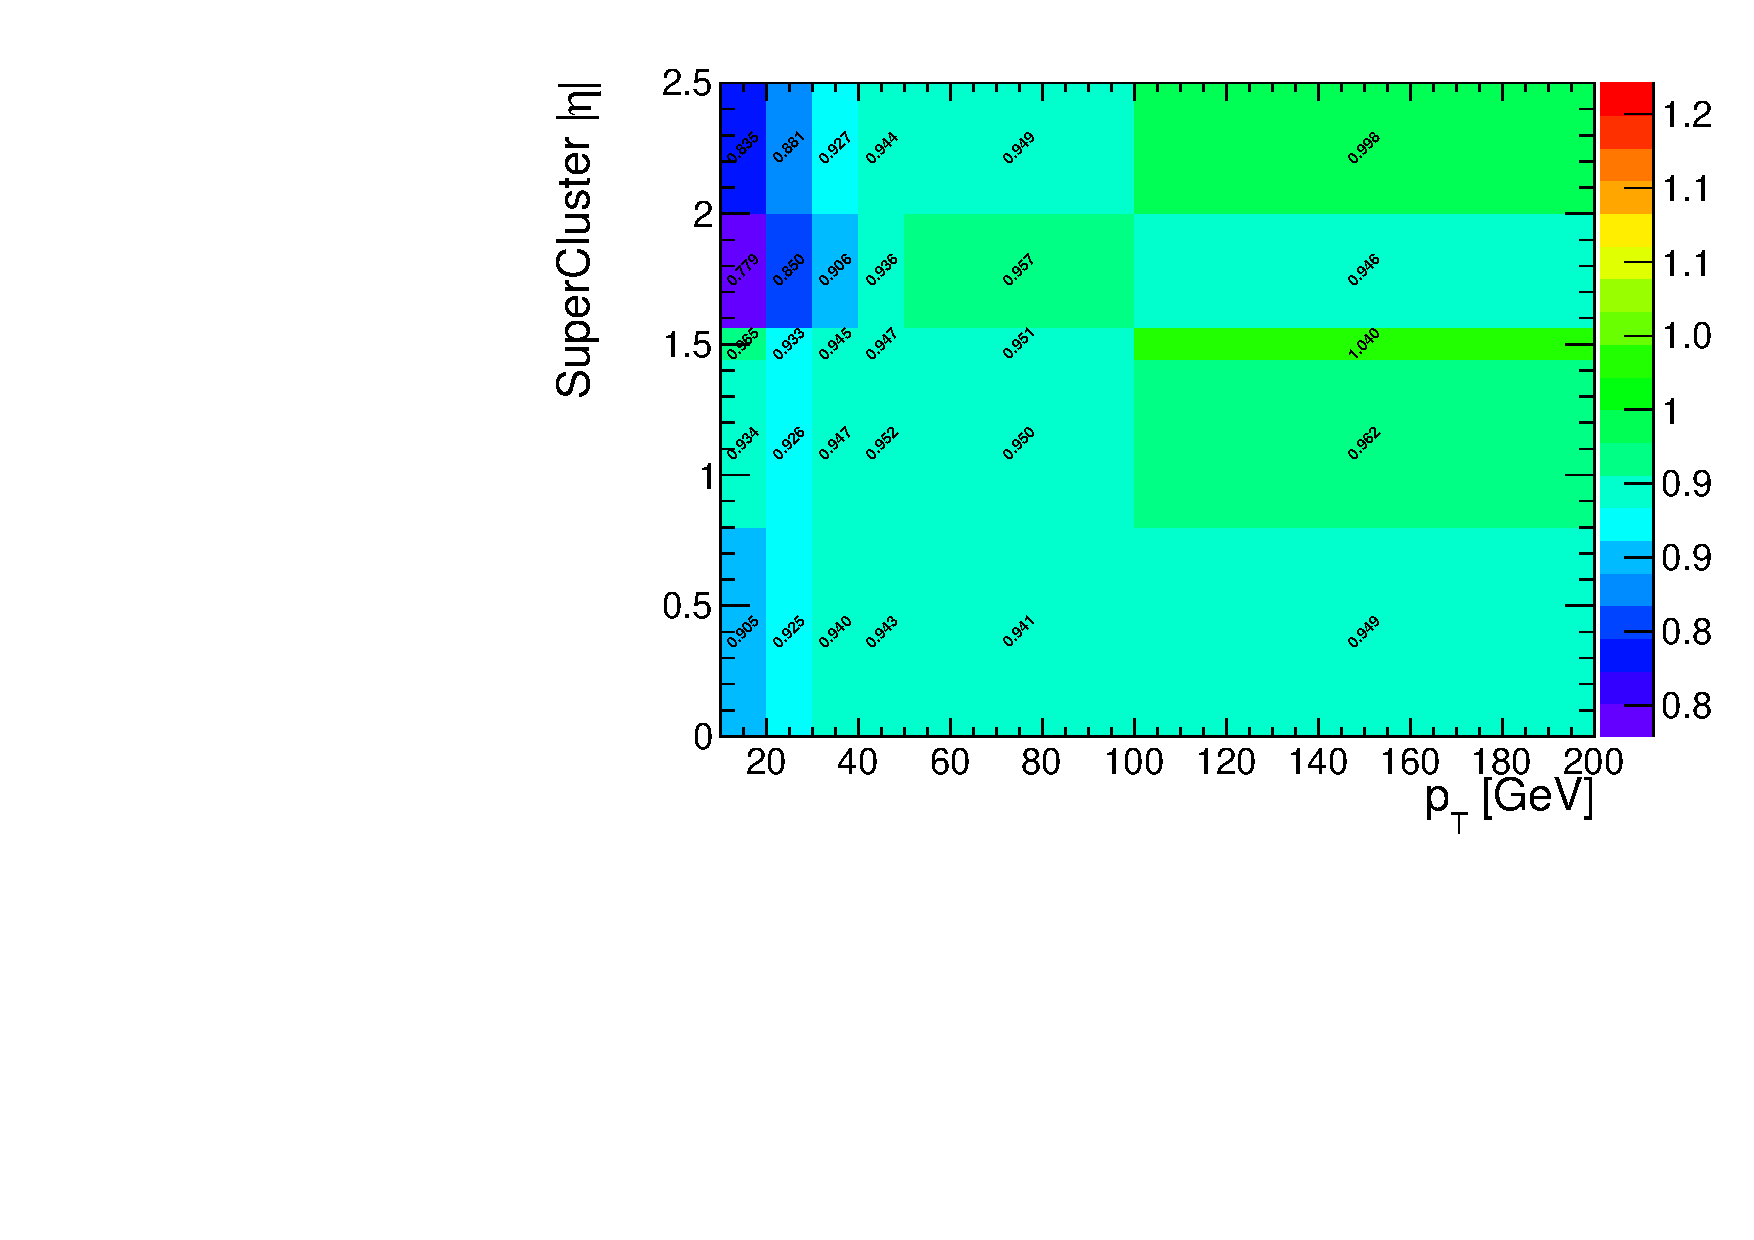
\includegraphics[width=0.45\textwidth]{figures/scaleFactors/GsfElectronToCutBasedStopsDilepton.pdf}}
	\subfloat[electron multi-isolation VT]{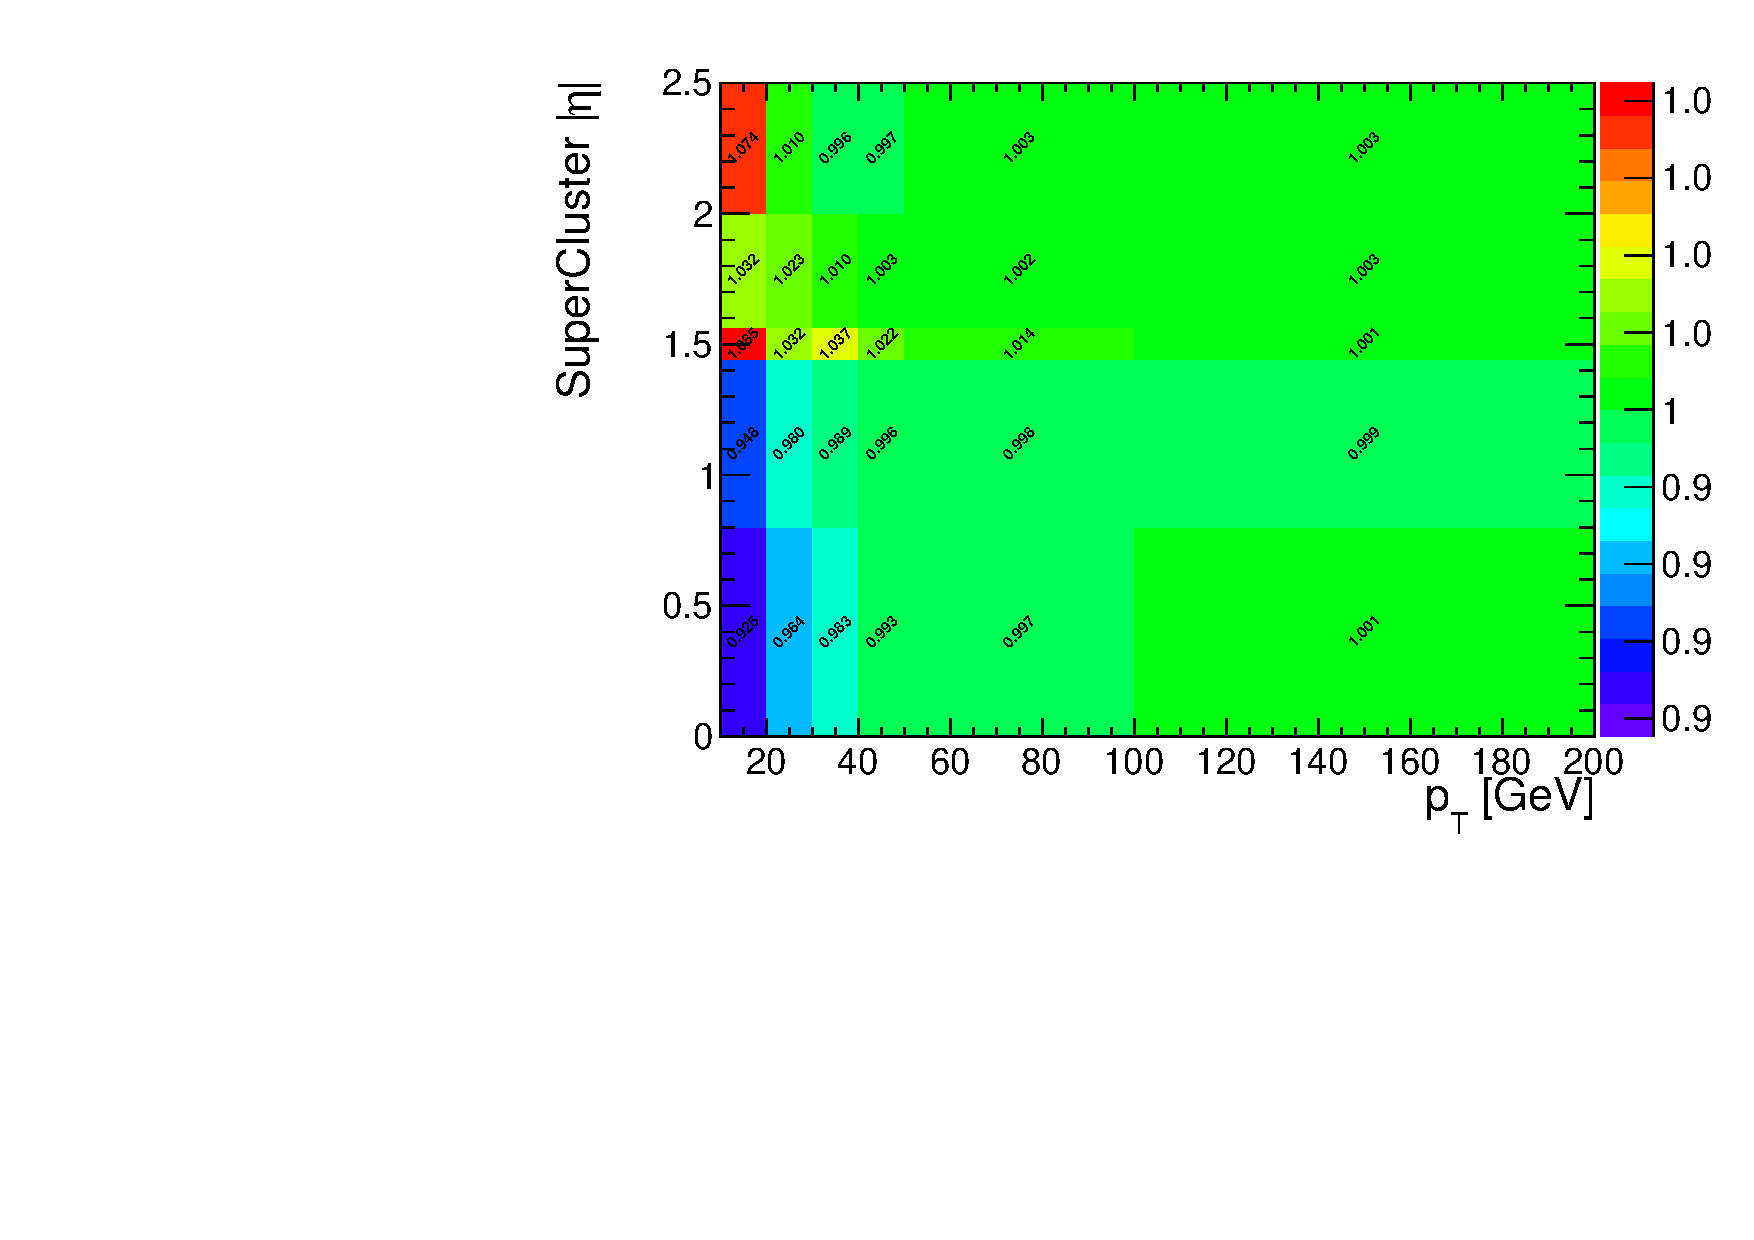
\includegraphics[width=0.45\textwidth]{figures/scaleFactors/CutBasedTightElectronToMultiIsoVT.pdf}}
	\caption{Scale factors for the identification and multi-isolation VT working point for electrons. Will be updated with final measurements.}
	\label{fig:SF_e}
      \end{figure}

  \subsection{Jet Selection}
  Particle candidates found by the PF algorithm are clustered into jets using the Anti-\kt algorithm \citep{Cacciari:2008gp} with distance parameter R = 0.4 (AK4). The influence of pileup
  is mitigated by the Charged Hadron Subtraction (CHS) technique which ignores charged particle candidates with a track closer along the $z$-axis to any vertex other than the main primary vertex. 
  Jets are calibrated in simulation and in data separately, accounting for deposits from pile-up and the imperfect detector response.
  Corrected jets with $p_{\mathrm{T}}> 30\,\GeV$ and $|\eta|<2.4$ are selected if they pass the loose jet identification criteria \citep{twiki:jetId}, i.e. the neutral electromagnetic and hadron fractions
  are $<99\%$ and the jet consists of at least two PF candidates. Furthermore, both the charged hadron fraction and multiplicity are required to be $>0$ and the charged electromagnetic fraction has to be $<99\%$.

  A selected jet may still overlap with the selected leptons.
  This is possible because the lepton can be clustered into a jet as well.
  To prevent such cases, jets that are found within a cone of $R=0.4$ around any of the selected signal leptons are  removed from the set of selected jets.

  Jets originating from the hadronization of $b$-quarks are identified using the Combined Secondary Vertex algorithm (CSVv2). The CSVv2 algorithm combines information from track impact parameters and secondary vertices identified within a given jet.
  In this analysis, a jet is $b$-tagged when its CSVv2 value passes the medium working point (\ie CSVv2 $>$ 0.800) \citep{twiki:btag}.

